% HIKET -- storyline v3. SECOND PASS, restructured onto the shape of the real paper.
%
% WHAT CHANGED vs v2 (built 2026-09-03 from Lorenzo's 19 PDF annotations on v2;
% the annotated original is revisions/HIKET_storyline_v2_annotated_20260903.pdf):
%   (1) OUTER SHELL IS NOW IMRaD. v2 was an arc; a journal wants Introduction /
%       Materials and methods / Results / Discussion / Conclusions. OCAR survives as
%       the INNER spine -- the arc now runs THROUGH the conventional sections rather
%       than replacing them. Schimel's point is that these are compatible; v2 simply
%       had not done the join.
%   (2) CONCLUSIONS EXIST. v2 ended on the policy deliverable, which Lorenzo flags as
%       "a nice bonus product", not a conclusion. Conclusions now return to the opening
%       questions and their resolutions, in the order of importance below.
%   (3) WEIGHTED, NOT BALANCED. Target: ~55% national trend, ~25% the ridge-position
%       side arc, ~20% unexplained local variance (and its last part very brief).
%   (4) LESS MODEL-ORIENTED. The biological content that the input result demands --
%       fine roots, exudates, mycorrhizae, pioneer vegetation, understorey -- is now a
%       section of its own rather than four lines inside a mechanism list.
%   (5) Claims softened where flagged: the observed rate is not treated as truth, the
%       "structural uncertainty" deliverable is walked back, the "surprise" is stated
%       once and not staged.
%
% NARRATIVE FRAMEWORKS (unchanged, see memory narrative-tools-ocar-jung):
%   OCAR -- now INTERNAL to IMRaD, signposted in source comments only.
%   Jungian archetypes -- HIDDEN, private map, must never surface in the text.
%   Gopen & Swan -- sentence level: old information first, payload in the stress position.
\documentclass[11pt]{article}
\usepackage[utf8]{inputenc}\usepackage[T1]{fontenc}
\usepackage[margin=2.4cm]{geometry}
\usepackage{graphicx}\usepackage{amsmath}\usepackage{amssymb}\usepackage{xcolor}
\usepackage{float}\usepackage[hidelinks]{hyperref}
\usepackage{caption}\captionsetup{font=small,labelfont=bf}
\usepackage[most]{tcolorbox}
\usepackage{tikz}\usetikzlibrary{positioning, arrows.meta, calc, fit, backgrounds}
\usepackage{titlesec}\usepackage{placeins}
\titlespacing*{\paragraph}{0pt}{0.9\baselineskip}{0.4em}
\setcounter{secnumdepth}{4}\setcounter{tocdepth}{2}

% --- STRUCTURAL TOGGLE ---------------------------------------------------
% \combinedtrue  = one "Results and Discussion" section (recommended, and what
%                  Lorenzo leaned toward). \combinedfalse = classic split.
% Nothing else changes; the same blocks are emitted either way.
\newif\ifcombined \combinedtrue

\definecolor{notebg}{HTML}{EAF2FB}\definecolor{noterule}{HTML}{2C6FB5}
\newtcolorbox{note}{colback=notebg, colframe=noterule, boxrule=0pt, leftrule=3pt,
  arc=1pt, left=8pt, right=8pt, top=5pt, bottom=5pt, fontupper=\small,
  before skip=7pt, after skip=7pt}
\definecolor{testbg}{HTML}{EAF7EE}\definecolor{testrule}{HTML}{2E8B57}
\newtcolorbox{test}{colback=testbg, colframe=testrule, boxrule=0pt, leftrule=3pt,
  arc=1pt, left=8pt, right=8pt, top=5pt, bottom=5pt, fontupper=\small,
  before skip=7pt, after skip=7pt}
\definecolor{warnbg}{HTML}{FDF3E3}\definecolor{warnrule}{HTML}{C08A2E}
\newtcolorbox{warn}{colback=warnbg, colframe=warnrule, boxrule=0pt, leftrule=3pt,
  arc=1pt, left=8pt, right=8pt, top=5pt, bottom=5pt, fontupper=\small,
  before skip=7pt, after skip=7pt}
\definecolor{lorbg}{HTML}{F3EDF9}\definecolor{lorrule}{HTML}{6B3FA0}
\newtcolorbox{ann}{colback=lorbg, colframe=lorrule, boxrule=0pt, leftrule=3pt,
  arc=1pt, left=8pt, right=8pt, top=5pt, bottom=5pt, fontupper=\small,
  before skip=7pt, after skip=7pt}

\newcommand{\sinit}{\sigma_{\mathrm{init}}}
\newcommand{\sinput}{\sigma_{\mathrm{input}}}

% --- figure embedding (same machinery as v2) -----------------------------
\graphicspath{{figures/}{../Reporting/NextgenC_report/SOC_maps/thumbnails/}}
\newcommand{\FIGlabel}[1]{\textcolor{noterule}{\small$\blacktriangleright$ \textsf{#1}}}
\newcommand{\FIG}{\begingroup\catcode`\_=12\relax\FIGaux}
\newcommand{\FIGaux}[1]{%
  \FIGlabel{#1}\endgroup
  \IfFileExists{figures/#1.png}{%
    \begin{figure}[htbp]\centering
      \includegraphics[width=0.92\linewidth,height=0.40\textheight,keepaspectratio]{figures/#1.png}
      \caption{\textsf{#1}}\end{figure}}{%
  \IfFileExists{figures/#1.tex}{%
    \begin{table}[htbp]\centering\scriptsize\input{figures/#1.tex}\end{table}}{%
  \IfFileExists{../Reporting/NextgenC_report/SOC_maps/thumbnails/#1.png}{%
    \begin{figure}[htbp]\centering
      \includegraphics[width=0.58\linewidth,height=0.42\textheight,keepaspectratio]{#1.png}
      \caption{\textsf{#1} (NextGenC deliverable)}\end{figure}}{%
  \textcolor{warnrule}{\small[\textsf{#1} --- FILE NOT FOUND]}}}}}
\newcommand{\FIGX}[1]{\textcolor{noterule}{\small$\blacktriangleright$ \textsf{#1}}}
\newcommand{\NEW}[1]{\textcolor{testrule}{\small$\bigstar$ \textsf{TO BUILD: #1}}}
\newcommand{\LIT}[1]{\textcolor{lorrule}{\small$\Box$ \textsf{LIT REVIEW: #1}}}

\title{\vspace{-1.4cm}\textbf{HIKET --- the storyline, v3}\\[2pt]
\large second pass: the arc fitted to the structure of the paper}
\author{}
\date{\small Version of \today. Numbers keyed to RUN\_IDs \texttt{20260831\_1624*} (arm B).
Built from the 19 annotations on v2 (\texttt{revisions/HIKET\_storyline\_v2\_annotated\_20260903.pdf}).}

\begin{document}\maketitle

\begin{note}
\textbf{How to read this.} The outer shell is now the conventional one --- Introduction,
Materials and methods, Results and Discussion, Conclusions --- because that is what the paper has to
be. \textbf{OCAR has not been abandoned; it has been moved inside.} The Opening and Challenge live in
the Introduction, the Action is the Methods, and the Resolution is distributed across the Results in
the order of importance set below. Each block is still one claim, its evidence, and nothing else.
\FIGX{name} marks a figure; \NEW{name} one still to build; \LIT{topic} a literature review that must
happen before the section can be written. Amber boxes are things that could sink a claim; green boxes
are tests we could run; \textcolor{lorrule}{\textbf{violet boxes carry Lorenzo's v2 annotations}} and
what was done about them.
\end{note}

% =====================================================================
% THE WEIGHT BUDGET. This is the single most consequential instruction from the
% v2 annotations: the paper is about the NATIONAL TREND, and everything else is
% subordinate. Drawn rather than stated so it cannot be forgotten while drafting.
% =====================================================================
\begin{center}
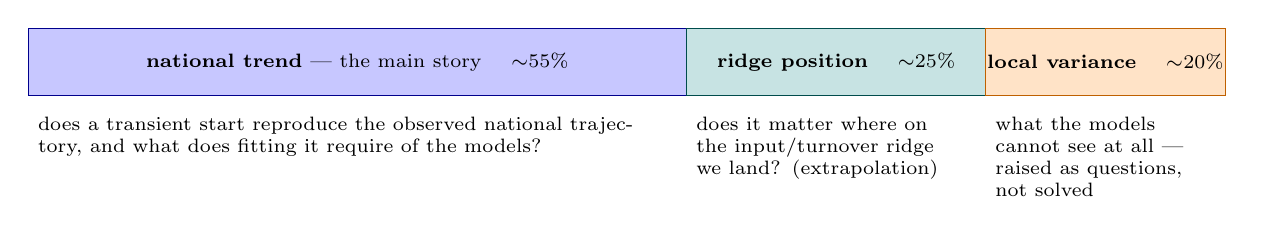
\begin{tikzpicture}[font=\scriptsize]
\def\W{15.2}
\fill[blue!22, draw=blue!55!black] (0,0) rectangle (0.55*\W,0.85);
\fill[teal!22, draw=teal!60!black] (0.55*\W,0) rectangle (0.80*\W,0.85);
\fill[orange!22, draw=orange!75!black] (0.80*\W,0) rectangle (\W,0.85);
\node at (0.275*\W,0.42) {\textbf{national trend} --- the main story \quad$\sim$55\%};
\node at (0.675*\W,0.42) {\textbf{ridge position} \quad$\sim$25\%};
\node at (0.90*\W,0.42) {\textbf{local variance} \quad$\sim$20\%};
\node[anchor=north west, text width=8.0cm, align=left] at (0,-0.15)
  {does a transient start reproduce the observed national trajectory, and what does
   fitting it require of the models?};
\node[anchor=north west, text width=3.4cm, align=left] at (0.55*\W,-0.15)
  {does it matter where on the input/turnover ridge we land? (extrapolation)};
\node[anchor=north west, text width=2.7cm, align=left] at (0.80*\W,-0.15)
  {what the models cannot see at all --- raised as questions, not solved};
\end{tikzpicture}
\end{center}

\begin{ann}
\textbf{Annotation (p17):} ``\emph{your draft is a lot on the model perspective but it will have to be
more anchored in biology in the end \dots\ weight is about 50--60\% general trends, 20--30\% this side
arc \dots\ remaining unexplained local variance and what we could do about it (very briefly the
last).}'' \textbf{Done:} the budget above governs this version, and the biological content that the
input result demands is now \S\ref{sec:missingflux} rather than four lines in a mechanism list.
\end{ann}

\tableofcontents
\bigskip

% =====================================================================
% INTRODUCTION.  OCAR's O and C live here. Lorenzo (p3): the problem, its meaning
% for the national GHG balance, and a brief look at the data belong at the FRONT.
% =====================================================================
\section{Introduction}

\subsection{A sink that appears to be levelling off}
\paragraph{What the inventory measures.} On the balanced plot set the mean stock runs
$64.5 \to 71.5 \to 73.6$~tC\,ha$^{-1}$ across the three campaigns: $+7.0$, then $+2.1$.
Accumulation, bending over. \FIG{F3_mean_soc}

\paragraph{The rate, and what it is a rate of.} $+0.259 \pm 0.040$~tC\,ha$^{-1}$\,yr$^{-1}$ over
1985--2024 on the balanced set, whole profile, true observation years. Over the last interval alone
it is $+0.117 \pm 0.066$ --- a confidence interval that includes zero.
\begin{ann}
\textbf{Annotation (p3): ``Which rate? And which report?''} \textbf{Fixed here:} the basis is now
stated wherever a rate appears (balanced set $n=310$, unweighted, whole profile, true years), because
the same data give $+0.209$ on the pairwise set --- a factor $1.8$ on the headline. The reporting
basis was decided on 2026-08-17 and every quoted rate in the paper must name it.
\end{ann}

\paragraph{Why the levelling-off is the interesting part.} A soil that is still accumulating and a
soil that has stopped are the same stock and different futures. The second derivative, not the
stock, is what an inventory projection turns on.

\begin{warn}
\textbf{Do not present the observed rate as truth} (annotation, p7). Three campaigns measured by
three protocols over four decades give a rate with a real and partly unquantified comparability
error: 1985 is a decade wide, its organic layer had to be reconstructed, and the short interval's
CI includes zero. The paper states what was measured and how, and treats agreement between models
and observations as consistency rather than as validation.
\end{warn}

\subsection{Why it matters for the national greenhouse gas balance}
\paragraph{The soil term is the uncertain one.} Finland's forest soil carbon flux enters the
national inventory, and whether it is a growing sink or a saturating one changes the reported
balance and the policy conclusions drawn from it. \LIT{the GHG inventory chain: how the soil term is
produced, reported and used; where our models sit in it}

\paragraph{What the inventory asks a model to do.} Not to rank plots, but to reproduce a national
trajectory over decades and project it forward. That is the quantity this paper evaluates, and
saying so early prevents a later result (near-zero plot-level skill) from reading as failure.

\subsection{The convention: soils initialised at steady state}
\paragraph{It is near-universal, and rarely examined.} The dominant practice across inventory
applications is to start the soil at the equilibrium implied by contemporary litter input.
\LIT{steady-state initialisation across model lineages --- Yasso, RothC, Century/DayCent, ICBM,
CBM-CFS3; how each initialises, and how often the assumption is tested}
\begin{ann}
\textbf{Annotation (p3, twice): ``This will need literature review across multiple model
lineages.''} \textbf{Acknowledged, not yet done} --- flagged here as a blocking dependency: the
claim of near-universality cannot be made without it.
\end{ann}

\paragraph{What steady state assumes.} \LIT{the theory paragraph (annotation, p5): what an
equilibrium state is for a linear donor-controlled system, what it assumes about the constancy of
inputs and climate, what properties follow --- $C=J/k$, the loss of all timing information, and the
fact that the assumption is about the \emph{history}, not about the soil}

\paragraph{And what follows from it.} An equilibrium start is already at the end of the accumulation.
It cannot produce a rise, so it cannot show a rise levelling off; the very dynamic the inventory
needs is the one the convention defines away.

\subsection{Finnish forests are a managed landscape, not an equilibrium one}
\paragraph{The history is the argument.} Exploitation, then a century of managed regrowth: growing
stock rose from roughly 1400 to 1775~million~m$^3$ between 1917 and 1985 and has risen further since.
A soil integrating a century of that is not at equilibrium with today's litter.
\FIG{F10b_forest_history}
\begin{ann}
\textbf{Annotation (p5): ``This is load bearing and will also need proper literature revision.''}
\textbf{Agreed --- and it is the load-bearing claim of the whole paper.} \LIT{Finnish forest
management history and its soil-carbon consequences; the non-equilibrium initialisation problem
(Peltoniemi 2004 as the direct antecedent); evidence on how long soils lag a change in input}
\end{ann}

\subsection{Objectives}
\paragraph{Three questions, in the order the paper weights them.}
(i) Does a transient, calibrated initialisation reproduce the observed national trajectory, and what
does reproducing it require of the models? (ii) Does it matter, for extrapolation, where the
calibration lands on the input/turnover trade-off? (iii) What is left that none of the models can
see, and what would it take to see it?

% =====================================================================
% MATERIALS AND METHODS. OCAR's Action. Kept deliberately short here -- the real
% M&M already exists in HIKET_main_manuscript.tex; this is the storyline view of it.
% =====================================================================
\section{Materials and methods}

\subsection{Data}
\paragraph{Plots and campaigns.} Finnish NFI/BioSoil/Komeetta permanent plots; three SOC campaigns
(1985--95, 2006, 2024); 456 calibration-ready plots, 1205 plot-year observations.

\paragraph{One homogenized SOC basis.} Organic plus mineral to a per-plot variable depth cap plus a
modelled deep tail, reproducing the official national stocks exactly. \FIG{F2_baseline}

\paragraph{Litter input.} The Tupek product, tree litter including harvest residues and natural
mortality, excluding understorey. \FIG{F1_inputs}

\subsection{The model ladder}
\paragraph{Six models, one to five pools.} SP1, TP2, TP3, Yasso07, Yasso15, Yasso20 --- the simple
models as an interpretable benchmark, the Yasso family as the operational standard.
\begin{ann}
\textbf{Annotation (p9):} ``\emph{we are not really doing any structural uncertainty work \dots\ We
have the simpler structures as a benchmark, mainly, with Yasso as the proven standard.}''
\textbf{Adopted:} the ladder is described as a benchmark design, and the word ``structural
uncertainty'' is used only where it is earned (the forward spread), never as a product claim.
\end{ann}

\subsection{Transient initialisation}
\paragraph{The start becomes a parameter.} Each draw spins up from 1917 under a reconstructed input
ramp and is carried forward through all three campaigns; $\sinit$ scales the 1917 input level.
\FIG{F4_initialization}

\subsection{A fair frame}
\paragraph{Equal information, not equal parameter count.} Yasso does not fit its decomposition rates,
so the simple models do not either: intrinsic rates are externally anchored (ICBM), humification
fractions are free, and every model calibrates the same auxiliary pair.

\subsection{Calibration and error model}
\paragraph{One likelihood, and it does not pretend plots are independent.} Log-normal, with region,
plot and campaign offsets marginalised at fixed variances.

\subsection{Analyses}
\paragraph{Three, matching the three objectives.} Posterior predictive over the observed window; a
forward experiment contrasting published and calibrated parameters under climate scenarios; and a
residual analysis against site covariates.

% =====================================================================
% RESULTS (and DISCUSSION). OCAR's Resolution, distributed by the weight budget.
% =====================================================================
\ifcombined
  \section{Results and discussion}
  \begin{note}
  \textbf{Combined, deliberately.} Every result here needs its interpretation immediately: the level
  agreement means nothing without the ridge, and the ridge means nothing without what it costs. A
  split version is one toggle away (\texttt{\textbackslash combinedfalse}) if a target journal
  requires it.
  \end{note}
\else
  \section{Results}
\fi

% ---------------------------------------------------------------- STRAND 1
\subsection*{\textsc{Strand 1 --- the national trajectory} \normalfont(\emph{$\sim$55\% of the paper})}
\addcontentsline{toc}{subsection}{Strand 1 --- the national trajectory (~55\%)}

\subsubsection{The models reach the observed levels}
\paragraph{No model sits more than $3.5$~tC\,ha$^{-1}$ from any campaign mean.} On the current
calibration the ensemble reproduces all three campaign levels.
\begin{ann}
\textbf{Annotation (p7): ``I don't get what this refers to.''} The v2 text pointed at a
``$26$~tC\,ha$^{-1}$ too high at 1985'' caveat that no reader could know about --- it was an internal
memory of an earlier run. \textbf{Deleted}; the sentence now states the present result only.
\end{ann}

\subsubsection{And they reproduce the rate, within the limits of the data}
\paragraph{The ensemble brackets the observed rate, and two members land on it.} Yasso07 $+0.258$ and
Yasso15 $+0.250$ against an observed $+0.259$; TP2 and TP3 run stronger, SP1 and Yasso20 weaker.
\FIG{F5_stock_change}
\begin{warn}
\textbf{Stated as consistency, not as validation} (annotation, p7). The observed rate carries its own
comparability error, so ``two models land on it'' is reported as what was seen, with the campaign
caveats attached, and no model is preferred on this basis.
\end{warn}

\subsubsection{The trajectory shape splits the ensemble three ways}
\paragraph{Three behaviours, and they are legible.} Yasso07 and Yasso15 rise and flatten; TP2 and TP3
rise and keep rising; SP1 and Yasso20 peak in the late 2000s and decline. The same split is visible
in the per-plot deliverable. \NEW{F3b --- trajectory shape, three groups, explicitly grouped}
\begin{ann}
\textbf{Annotation (p7): ``Try it, but then we have to look at it together before including; current
Fig 6 in this text could be enough already.''} \textbf{Kept as \texttt{TO BUILD}} --- and note that
the grouping is already visible without a new figure in the NextGenC trajectory panel, which may
make F3b unnecessary. Decide when it exists.
\end{ann}

\subsubsection{This is what an equilibrium start forecloses}
\paragraph{The shape is the point.} Accumulation bending over is a statement about timing, and timing
is precisely what an equilibrium initialisation discards. Reproducing it is the paper's first result.

\subsubsection{Structure is nearly invisible in fit}
\paragraph{Skill does not climb the pool ladder.} Calibration $R^2$ $0.016$--$0.021$; holdout
$R^2 \le 0.0012$; holdout RMSE spans $3.6\%$, and the best and worst belong to a five-pool and a
three-pool model. \FIG{T1_model_summary} \FIG{F6b_skill_vs_complexity}

\paragraph{So fit cannot arbitrate between these structures.} Whatever separates them, it is not the
calibration data.

\subsubsection{The data pin a level, and little else}
\paragraph{Convergence is not identifiability.} R-hat $\le 1.008$ everywhere, yet the transfer
fractions are prior-pinned, ridge-correlated and carry under a nat.
\FIG{F8b_fraction_ridges} \FIG{F6_obs_vs_pred_holdout}

\subsubsection{What fitting the trajectory requires: more input, and faster turnover}
\paragraph{The calibration lands away from the published parameterisations.} Effective litter flux
$3.19$--$4.34$~tC\,ha$^{-1}$\,yr$^{-1}$, and intrinsic MRT $24.6$ / $27.1$ / $22.6$~yr for
Yasso07/15/20 against published $33.5$ / $30.5$ / $22.1$. \FIG{F12_mrt_yasso}

\paragraph{These are one displacement, not two.} The level constrains
$\mathrm{MRT} \times \sinput$, so faster-with-more and slower-with-less fit alike; the posterior
rides that ridge. \FIG{F14_mrt_ridge} \FIG{S13_mrt_ridge_benchmark}

\begin{ann}
\textbf{Annotation (p12), on ``a steady-state start hides exactly this'':} ``\emph{Steady state still
has the same problem of equifinality \dots\ with the trajectories the ridge on the likelihood surface
should narrow a bit \dots\ no need to overdo this surprise thing.}'' \textbf{Rewritten.} The claim is
now the weaker and defensible one: \emph{the ridge exists under either initialisation; a transient
start narrows it, because the approach rate carries information the equilibrium condition discards.}
Measured, the narrowing is partial --- MRT and $\sinput$ still correlate $-0.64$ to $-0.73$. The
``surprise'' framing is gone; the displacement is reported as a result, once.
\end{ann}

\begin{ann}
\textbf{Annotation (p12), on Liski: ``I don't think so, we are correcting even higher.''}
\textbf{Confirmed and corrected.} Liski 2006 implies $\sinput \approx 1.27$; our effective correction
runs $1.27$--$1.73$ across the six. Liski is the \textbf{floor} of our range, not a match --- so the
sentence becomes ``an independent estimate from the same country, period and model family sits at
the bottom of the range we infer'', which is a weaker corroboration and an honest one.
\end{ann}

\subsubsection{What might be missing from the input flux}\label{sec:missingflux}
\begin{ann}
\textbf{Annotation (p12), the longest one:} ``\emph{The input functions have a lot of trust in the
field \dots\ they do work (I think because the previous fitting compensates) \dots\ there needs to be
a very extensive review of the supporting evidence, with hypotheses well grounded in literature about
what we might be missing in the fluxes (first things to examine are fine root MRT, exudates and
mycorrhizae) \dots\ also missing pioneer vegetation.}'' \textbf{This section is the answer to that
note, and it is the main place where the paper stops being about models.}
\end{ann}

\paragraph{The candidate is not that the litter model is wrong, but that it is incomplete.} Litter
input products are trusted because they have worked for decades --- and one reason they work is that
a calibration free to adjust rates can absorb a missing flux without visible misfit. A transient
calibration on a fixed rate anchor removes that compensation, and what is missing then has to appear
somewhere.

\paragraph{Belowground turnover.} Fine root lifespan is the largest single lever on belowground
litter and is poorly constrained. \LIT{fine root MRT in boreal conifers: isotopic vs minirhizotron
estimates, and the factor-of-several disagreement between methods}

\paragraph{Rhizodeposition.} Exudates bypass the litter pathway entirely and are absent from
inventory litter models by construction. \LIT{exudate fluxes as a fraction of NPP in boreal forest}

\paragraph{Mycorrhizal necromass.} Increasingly implicated as a dominant precursor of stable soil
carbon in boreal systems, and entirely outside the litter product. \LIT{mycorrhizal contribution to
boreal SOC formation --- the Clemmensen line of evidence and what has followed it}

\paragraph{Understorey.} Excluded from the product by construction, and its share rises strongly
toward the north --- so a single national multiplier must be wrong in opposite directions at the two
ends of the country. \FIG{SX_input_vs_literature}

\paragraph{Early-succession vegetation.} Pioneer species after disturbance contribute litter that
inventory-based models, keyed to standing merchantable biomass, do not represent.
\LIT{pioneer/early-succession litter contributions after clear-cut and after fire}

\begin{warn}
\textbf{This section must not become an argument that we are right.} Each mechanism is a hypothesis
for where an apparently missing flux could come from, and several are not separable with our data.
The honest form is: the calibration says the input is larger than the product; here are physically
plausible sources; testing them is not this paper's job.
\end{warn}

% ---------------------------------------------------------------- STRAND 2
\subsection*{\textsc{Strand 2 --- does ridge position matter?} \normalfont(\emph{$\sim$25\%})}
\addcontentsline{toc}{subsection}{Strand 2 --- does ridge position matter? (~25\%)}

\begin{ann}
\textbf{Annotation (p17): ``For what? Do you mean if it has consequences for extrapolation, for
example?''} \textbf{Yes --- and the section is now titled that way.} v2's ``does the ridge position
matter?'' left the reader to guess the predicate. It matters \emph{for extrapolation}: two
calibrations that fit the observed window identically can project differently.
\end{ann}

\subsubsection{The question the ridge forces}
\paragraph{The data cannot choose a point on the ridge, so the choice must be judged by its
consequences.} If moving along it changes nothing we can observe, the displacement is bookkeeping.
If it changes the projection, it is a result with consequences for anyone using these models.

\subsubsection{The test: published parameters against ours, forward only}
\paragraph{No re-calibration, one input parameter refitted.} Both arms are pushed through the same
machinery under ramped scenarios; both match the observed window at least as well as each other, so
any divergence afterwards is extrapolation. \FIG{F15_forward_arms}

\subsubsection{It matters for one structure and not the others}
\paragraph{Only Yasso07 separates.} $-2.08$ $[-3.57, -0.79]$~tC\,ha$^{-1}$ at SSP2-4.5; Yasso15 and
Yasso20 do not separate at all.

\paragraph{And the mechanism is structural.} Yasso07 applies a single climate modifier to every pool,
so turnover and temperature sensitivity are tied to the same parameter and moving along the ridge
moves both. Yasso15 and Yasso20 carry pool-specific modifiers, and the pools that \emph{hold} the
carbon respond almost identically in both arms. \FIG{A1_forward_appendix}

\paragraph{The framing that survives.} Yasso15 and Yasso20 are not shown to be right; they are shown
to be \textbf{resilient} to an input assumption the data cannot settle. That is a usable statement
for an inventory, and a narrower one than ``our calibration changes the forecast''.

\begin{warn}
\textbf{The main forecast contains no climate change, and the paper must say so.} The projection
recycles the last twenty observed years and freezes litter at 2024, so its sink is relaxation toward
equilibrium, not a response. The scenarios appear only in this side arc, as an instrument for testing
ridge position. Doing it properly would need productivity to respond to warming as well.
\end{warn}

% ---------------------------------------------------------------- STRAND 3
\subsection*{\textsc{Strand 3 --- what none of the models can see} \normalfont(\emph{$\sim$20\%, and the last part brief})}
\addcontentsline{toc}{subsection}{Strand 3 --- what none of the models can see (~20\%)}

\begin{ann}
\textbf{Annotations (p16, two):} ``\emph{This seems about local variance, point variance, rather than
the overall trend \dots\ This is a separated topic. I would put it lower in priority \dots\ we are
just offering this analysis to raise new research questions \dots\ Our main story is about the global,
national variance.}'' \textbf{Restructured accordingly:} this is no longer a subsection inside the
input argument (where v2 put it, and where it did read as evidence for the input claim). It is its
own strand, last, at $\sim$20\%, and it is framed as a question raised rather than a gap filled.
\end{ann}

\subsubsection{The models order the national trajectory but not the plots}
\paragraph{Two statements that read as a contradiction only if separated.} The ensemble reproduces
the national mean trajectory and explains almost none of the between-plot variance. Both are true,
and the second is a statement about spatial resolution, not about the trajectory.

\subsubsection{What is left behind is recoverable, not irreducible}
\paragraph{Roughly half of the residual variance is predictable from covariates already in hand.} A
random forest on site variables explains $44$--$65\%$ of what the models leave (out-of-bag), with
observation reliability around $0.49$ --- so this is not a noise ceiling. \FIG{F11_rf_heatmap}

\paragraph{The same covariates lead in all six models.} Stand basal area first, then development
class and coarse-fragment content; the importance is diffuse rather than concentrated in one term.

\subsubsection{What that suggests, briefly}
\paragraph{Two of the leaders are productivity proxies and one is soil-physical.} A productivity
proxy leading everywhere is what a spatially varying input level would look like; a soil-physical
variable leading is something no model in the ensemble has a term for. \textbf{We name the
observation and stop there} --- the method that would exploit it is not this paper's to choose.

% =====================================================================
\section{Conclusions}
\begin{ann}
\textbf{Annotation (p22): ``The policy deliverable should not be a real conclusion, it is more a nice
bonus product. The conclusions \dots\ are more about the opening stories, their resolutions.''}
\textbf{Rebuilt exactly that way:} the conclusions below answer the three opening questions in the
order of the weight budget, and the deliverable is demoted to a closing paragraph.
\end{ann}

\paragraph{A transient, calibrated start reproduces a dynamic the conventional one cannot.} The
observed accumulation and its levelling-off are recovered by all six models at the level and by the
ensemble in rate, which an equilibrium initialisation forecloses by construction.

\paragraph{Reproducing it requires more litter input, and faster turnover, than the published
parameterisations carry.} These are one displacement along a trade-off the data cannot resolve, and
the most plausible reading is not that the models are wrong but that the input flux is incomplete ---
with belowground and non-tree sources the candidates.

\paragraph{Where the calibration lands on that trade-off reaches the projection, but only for some
structures.} A single climate modifier ties turnover to temperature sensitivity; pool-specific
modifiers do not. Models of the second kind are more robust to an assumption that cannot currently be
tested.

\paragraph{And a large, recoverable part of the plot-scale variance is invisible to every model
here.} It is a well-posed question for the next study rather than a limitation of this one.

\paragraph{Bonus product, not conclusion: the maps.} The calibrated ensemble yields gridded SOC and
its uncertainty for Finland, which is useful to the inventory and is offered as a deliverable rather
than as the paper's finding. \FIG{ENSEMBLE_SOC_mean}

% =====================================================================
\section*{Open decisions and what is still missing}
\addcontentsline{toc}{section}{Open decisions and what is still missing}

\paragraph{Structural.} Whether Results and Discussion stay combined (currently yes). Whether F3b is
built or the NextGenC panel suffices. Whether the arc diagram's thread vocabulary is retired.

\paragraph{Blocking literature reviews.} Steady-state initialisation across model lineages; the
theory of equilibrium initialisation; Finnish management history; and the whole of
\S\ref{sec:missingflux} --- fine root MRT, exudates, mycorrhizal necromass, pioneer vegetation.

\paragraph{Still not started.} Citations and a \texttt{.bib}; title and abstract; the coauthor block;
figure placement in the manuscript.

\paragraph{Unresolved from earlier sessions.} The 1917 stock floor is still an unsourced placeholder,
and the relaunch of the six calibrations after the Fortran guard change has not been done.

\end{document}
